


\tikzset{every picture/.style={line width=0.75pt}} %set default line width to 0.75pt        

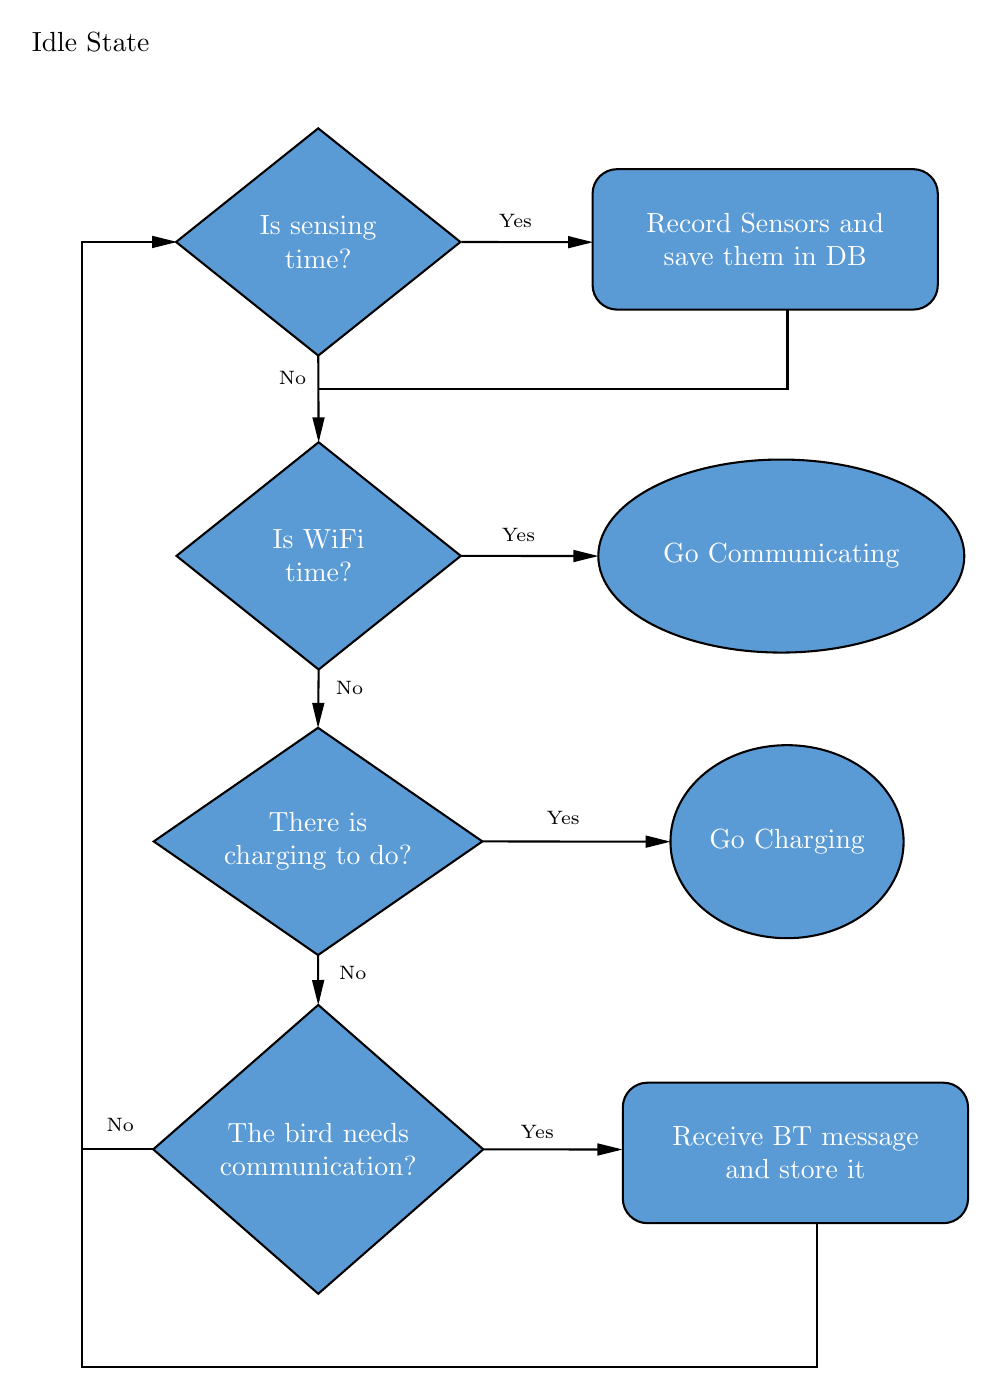
\begin{tikzpicture}[x=0.75pt,y=0.75pt,yscale=-1,xscale=1]
%uncomment if require: \path (0,690); %set diagram left start at 0, and has height of 690

%Flowchart: Decision [id:dp7566185043284532] 
\draw  [fill={rgb, 255:red, 91; green, 155; blue, 213 }  ,fill opacity=1 ] (150.5,63) -- (219,117.75) -- (150.5,172.5) -- (82,117.75) -- cycle ;
%Flowchart: Decision [id:dp5066246179354095] 
\draw  [fill={rgb, 255:red, 91; green, 155; blue, 213 }  ,fill opacity=1 ] (150.69,214.24) -- (219.19,268.99) -- (150.69,323.74) -- (82.19,268.99) -- cycle ;
%Flowchart: Decision [id:dp9002091770215006] 
\draw  [fill={rgb, 255:red, 91; green, 155; blue, 213 }  ,fill opacity=1 ] (150.4,351.81) -- (229.57,406.56) -- (150.4,461.31) -- (71.24,406.56) -- cycle ;
%Flowchart: Decision [id:dp28266720083320807] 
\draw  [fill={rgb, 255:red, 91; green, 155; blue, 213 }  ,fill opacity=1 ] (150.5,485.33) -- (230,554.92) -- (150.5,624.5) -- (71,554.92) -- cycle ;
%Flowchart: Alternative Process [id:dp4519956516169352] 
\draw  [fill={rgb, 255:red, 91; green, 155; blue, 213 }  ,fill opacity=1 ] (282.67,94.51) .. controls (282.67,87.97) and (287.97,82.67) .. (294.51,82.67) -- (437.16,82.67) .. controls (443.7,82.67) and (449,87.97) .. (449,94.51) -- (449,138.49) .. controls (449,145.03) and (443.7,150.33) .. (437.16,150.33) -- (294.51,150.33) .. controls (287.97,150.33) and (282.67,145.03) .. (282.67,138.49) -- cycle ;
%Shape: Ellipse [id:dp018827657637768613] 
\draw  [fill={rgb, 255:red, 91; green, 155; blue, 213 }  ,fill opacity=1 ] (320.19,406.69) .. controls (320.19,381.01) and (345.34,360.19) .. (376.36,360.19) .. controls (407.38,360.19) and (432.52,381.01) .. (432.52,406.69) .. controls (432.52,432.37) and (407.38,453.19) .. (376.36,453.19) .. controls (345.34,453.19) and (320.19,432.37) .. (320.19,406.69) -- cycle ;
%Flowchart: Alternative Process [id:dp0005817544992761103] 
\draw  [fill={rgb, 255:red, 91; green, 155; blue, 213 }  ,fill opacity=1 ] (297.24,534.65) .. controls (297.24,528.11) and (302.54,522.81) .. (309.08,522.81) -- (451.73,522.81) .. controls (458.27,522.81) and (463.57,528.11) .. (463.57,534.65) -- (463.57,578.63) .. controls (463.57,585.17) and (458.27,590.48) .. (451.73,590.48) -- (309.08,590.48) .. controls (302.54,590.48) and (297.24,585.17) .. (297.24,578.63) -- cycle ;
%Shape: Ellipse [id:dp5629079222432349] 
\draw  [fill={rgb, 255:red, 91; green, 155; blue, 213 }  ,fill opacity=1 ] (285.43,269.07) .. controls (285.43,243.39) and (324.9,222.57) .. (373.6,222.57) .. controls (422.29,222.57) and (461.76,243.39) .. (461.76,269.07) .. controls (461.76,294.75) and (422.29,315.57) .. (373.6,315.57) .. controls (324.9,315.57) and (285.43,294.75) .. (285.43,269.07) -- cycle ;
%Straight Lines [id:da3966705421008925] 
\draw    (219.4,117.75) -- (280.83,117.85) ;
\draw [shift={(282.83,117.86)}, rotate = 180.1] [fill={rgb, 255:red, 0; green, 0; blue, 0 }  ][line width=0.08]  [draw opacity=0] (12,-3) -- (0,0) -- (12,3) -- cycle    ;
%Straight Lines [id:da846839102506278] 
\draw    (150.5,172.5) -- (150.68,212.24) ;
\draw [shift={(150.69,214.24)}, rotate = 269.74] [fill={rgb, 255:red, 0; green, 0; blue, 0 }  ][line width=0.08]  [draw opacity=0] (12,-3) -- (0,0) -- (12,3) -- cycle    ;
%Shape: Right Angle [id:dp6571215182174597] 
\draw   (376.57,150.71) -- (376.57,188.71) -- (151,188.71) ;
%Straight Lines [id:da8394296462529047] 
\draw    (219.19,268.99) -- (283.43,269.07) ;
\draw [shift={(285.43,269.07)}, rotate = 180.07] [fill={rgb, 255:red, 0; green, 0; blue, 0 }  ][line width=0.08]  [draw opacity=0] (12,-3) -- (0,0) -- (12,3) -- cycle    ;
%Straight Lines [id:da4710885721141074] 
\draw    (150.69,323.74) -- (150.43,349.81) ;
\draw [shift={(150.4,351.81)}, rotate = 270.58] [fill={rgb, 255:red, 0; green, 0; blue, 0 }  ][line width=0.08]  [draw opacity=0] (12,-3) -- (0,0) -- (12,3) -- cycle    ;
%Straight Lines [id:da4248251640374108] 
\draw    (229.57,406.56) -- (318.19,406.69) ;
\draw [shift={(320.19,406.69)}, rotate = 180.08] [fill={rgb, 255:red, 0; green, 0; blue, 0 }  ][line width=0.08]  [draw opacity=0] (12,-3) -- (0,0) -- (12,3) -- cycle    ;
%Straight Lines [id:da4740933242173315] 
\draw    (150.4,461.31) -- (150.49,483.33) ;
\draw [shift={(150.5,485.33)}, rotate = 269.77] [fill={rgb, 255:red, 0; green, 0; blue, 0 }  ][line width=0.08]  [draw opacity=0] (12,-3) -- (0,0) -- (12,3) -- cycle    ;
%Straight Lines [id:da6570962624535117] 
\draw    (230,554.92) -- (295,555) ;
\draw [shift={(297,555)}, rotate = 180.07] [fill={rgb, 255:red, 0; green, 0; blue, 0 }  ][line width=0.08]  [draw opacity=0] (12,-3) -- (0,0) -- (12,3) -- cycle    ;
%Shape: Right Angle [id:dp9183066958097172] 
\draw   (71,554.92) -- (36.6,554.92) -- (36.6,117.29) ;
%Shape: Right Angle [id:dp3632444516031996] 
\draw   (390.8,590.1) -- (390.8,660) -- (36.2,660) ;
%Straight Lines [id:da19159223364389222] 
\draw    (36.6,554.92) -- (36.6,660) ;
%Straight Lines [id:da3039240044456082] 
\draw    (37,117.75) -- (80.4,117.75) ;
\draw [shift={(82.4,117.75)}, rotate = 180] [fill={rgb, 255:red, 0; green, 0; blue, 0 }  ][line width=0.08]  [draw opacity=0] (12,-3) -- (0,0) -- (12,3) -- cycle    ;

% Text Node
\draw (11,15) node [anchor=north west][inner sep=0.75pt]   [align=left] {Idle State};
% Text Node
\draw (150.5,117.75) node   [align=left] {\begin{minipage}[lt]{48.65pt}\setlength\topsep{0pt}
\begin{center}
\textcolor[rgb]{1,1,1}{Is sensing}\\\textcolor[rgb]{1,1,1}{time?}
\end{center}

\end{minipage}};
% Text Node
\draw (150.69,268.99) node   [align=left] {\begin{minipage}[lt]{33.88pt}\setlength\topsep{0pt}
\begin{center}
\textcolor[rgb]{1,1,1}{Is WiFi}\\\textcolor[rgb]{1,1,1}{time?}
\end{center}

\end{minipage}};
% Text Node
\draw (150.4,406.56) node   [align=left] {\begin{minipage}[lt]{73.05pt}\setlength\topsep{0pt}
\begin{center}
\textcolor[rgb]{1,1,1}{There is}\\\textcolor[rgb]{1,1,1}{charging to do?}
\end{center}

\end{minipage}};
% Text Node
\draw (150.5,554.92) node   [align=left] {\begin{minipage}[lt]{76.99pt}\setlength\topsep{0pt}
\begin{center}
\textcolor[rgb]{1,1,1}{The bird needs}\\\textcolor[rgb]{1,1,1}{communication?}
\end{center}

\end{minipage}};
% Text Node
\draw (365.83,116.5) node   [align=left] {\begin{minipage}[lt]{95.71pt}\setlength\topsep{0pt}
\begin{center}
\textcolor[rgb]{1,1,1}{Record Sensors and}\\\textcolor[rgb]{1,1,1}{save them in DB}
\end{center}

\end{minipage}};
% Text Node
\draw (380.4,556.64) node   [align=left] {\begin{minipage}[lt]{99.48pt}\setlength\topsep{0pt}
\begin{center}
\textcolor[rgb]{1,1,1}{Receive BT message}\\\textcolor[rgb]{1,1,1}{and store it}
\end{center}

\end{minipage}};
% Text Node
\draw (376.36,406.69) node  [color={rgb, 255:red, 255; green, 255; blue, 255 }  ,opacity=1 ] [align=left] {Go Charging};
% Text Node
\draw (373.6,269.07) node  [color={rgb, 255:red, 255; green, 255; blue, 255 }  ,opacity=1 ] [align=left] {Go Communicating};
% Text Node
\draw (47,538.5) node [anchor=north west][inner sep=0.75pt]  [font=\scriptsize] [align=left] {No};
% Text Node
\draw (130,178.6) node [anchor=north west][inner sep=0.75pt]  [font=\scriptsize] [align=left] {No};
% Text Node
\draw (157.5,328.1) node [anchor=north west][inner sep=0.75pt]  [font=\scriptsize] [align=left] {No};
% Text Node
\draw (159,465) node [anchor=north west][inner sep=0.75pt]  [font=\scriptsize] [align=left] {No};
% Text Node
\draw (236,103.1) node [anchor=north west][inner sep=0.75pt]  [font=\scriptsize] [align=left] {Yes};
% Text Node
\draw (237.5,254.1) node [anchor=north west][inner sep=0.75pt]  [font=\scriptsize] [align=left] {Yes};
% Text Node
\draw (259,390.5) node [anchor=north west][inner sep=0.75pt]  [font=\scriptsize] [align=left] {Yes};
% Text Node
\draw (246.5,542) node [anchor=north west][inner sep=0.75pt]  [font=\scriptsize] [align=left] {Yes};


\end{tikzpicture}